\section{Mini Projet - Programmation noyau et système}
\subsection{Travail à réaliser}
Concevez une application permettant de gérer automatiquement et manuellement la vitesse de rotation du ventilateur de l'Odroid-XU3 Lite.\\
Cette application réalisera la fonctionnalité minimale suivante:
\begin{enumerate}
	\item La supervision de la température du microprocesseur et la gestion automatique de la vitesse du ventialteur devront être réalisées par un module noyau. Ce module devra offrir via le sysfs une interface permettant de choisir:
	\begin{itemize}
		\item le mode automatique ou manuel
		\item le duty cycle à appliquer au PWM en mode manuel
	\end{itemize}
	\item La gestion du mode manuel devra être implémentée par un deamon en espace utilisateur. Ce deamon proposera deux interfaces distinctes:
	\begin{enumerate}
		\item Interface physique via les boutons poussoir et LEDs de la carte d'extension
		\begin{itemize}
			\item SW1 pour augmenter la vitesse de rotation du ventilateur, la pression du SW1 devra être signalisée sur la LED1
			\item SW2 pour diminuer la vitesse de rotation du ventilateur, la pression du SW2 devra être signalisée sur la LED2
			\item SW3 pour changer du mode automatique au mode manuel et vice versa. Le mode manuel sera signalé avec la LED3 allumée
		\end{itemize}
		\item Interface IPC au choix du développeur permettant de dialoguer avec une application pour choisir le mode de fonctionnement et spécifier la valeur du duty cycle
	\end{enumerate}
	\item Selon le choix de l'interface IPC, une petite application implémentant une interface utilisateur pour piloter le ventilateur via le deamon devra être réalisée.
\end{enumerate}
\subsection{Installation des différentes parties}
Le miniprojet est constituer d'un module noyau, d'un daemon et d'une application utilisateur, voici les différentes étapes pour les installer. Il faut bien évidement que chaque partie aie été préalablement compilée.
\subsubsection{Daemon}
\textbf{Emplacement du code: }\textit{/miniprojet/daemon/}\\
\begin{lstlisting}
//Install
# cp /usr/workspace/csel1/environment/miniProjet/daemon/S70appl /etc/init.d/
# reboot

//Uninstall
# rm /etc/init.d/S70appl
# reboot
\end{lstlisting}
\subsubsection{Module noyau}
\textbf{Emplacement du code: }\textit{/miniprojet/module\_noyau/}\\
\begin{lstlisting}
//Install
# modprobe mymodule

//Uninstall
# modprobe -r mymodule
\end{lstlisting}
\subsubsection{Application utilisateur}
\textbf{Emplacement du code: }\textit{/miniprojet/user/}\\
\begin{lstlisting}
# cd /usr/workspace/csel1/environment/miniProjet/user/
# ./app_h 
\end{lstlisting}
\subsection{Daemon en espace utilisateur}
Le daemon se lance automatiquement au démarrage de l'ODROID s'il a été correctement installé. Ses messages ont été redirigés dans le syslog. On peut les voir à l'aide des commandes suivantes:
\begin{lstlisting}
//Pour voir les derniers messages
# cat /var/log/messages | tail -f

//ou pour afficher les messages en temps reel
# tail -f /var/log/messages

Jan  1 04:54:23 odroidxu3 daemon.info app_a[1620]: Daemon Mode manual
Jan  1 04:54:23 odroidxu3 user.info kernel: [ 1941.377057] [c5] Fan Control : changed mode to manual
Jan  1 04:54:23 odroidxu3 user.info kernel: [ 1941.380725] [c5] Duty set to : 10486
Jan  1 04:54:24 odroidxu3 daemon.info app_a[1620]: daemon Duty 48
Jan  1 04:54:24 odroidxu3 user.info kernel: [ 1942.920102] [c5] Fan Control : duty of 48 trying to be set
Jan  1 04:54:24 odroidxu3 user.info kernel: [ 1942.924106] [c5] Fan Control : duty of 48 was set
Jan  1 04:54:24 odroidxu3 user.info kernel: [ 1942.928857] [c5] Duty set to : 10066
Jan  1 04:54:25 odroidxu3 daemon.info app_a[1620]: daemon Duty 50
Jan  1 04:54:25 odroidxu3 user.info kernel: [ 1943.713271] [c5] Fan Control : duty of 50 trying to be set
Jan  1 04:54:25 odroidxu3 user.info kernel: [ 1943.717325] [c5] Fan Control : duty of 50 was set
Jan  1 04:54:25 odroidxu3 user.info kernel: [ 1943.722008] [c5] Duty set to : 10486
Jan  1 04:54:27 odroidxu3 daemon.info app_a[1620]: daemon Duty 48
\end{lstlisting}

À l'aide des boutons de la carte d'extension, on peut gérer le duty cycle du ventilateur et le mode manual/auto. Le duty cycle du ventilateur n'est modifié que lorsque l'on est en mode manuel (option du module noyau). Les LEDs s'allument en fonction de la pression sur les boutons.\\
Une option a été ajoutée au cahier des charges. Quand on tient longtemps un bouton appuyé, le duty cycle s'auto incrémente.\\
L'IPC choisi est un fifo entre l'application utilisateur et le daemon.\\
Le daemon contient deux processus, un pour les boutons, l'autre pour l'IPC.\\
\textbf{Warning: } Contrairement à l'exemple des slides, le "passwd" pour donner les droits a du être changé à "root" au lieu de "daemon", car les gpio sont importées/exportées après l'initialisation dans le daemon body. Normalement, cette action devrait être faite avant.

\subsection{Module de contrôle du ventilateur}
Comme le module doit proposer une interface dans le sysfs permettant de régler le mode de fonctionnement et la vitesse en cas de mode manuel, deux fichiers d'attributs ont été créés:
\begin{itemize}
	\item duty : permet, en mode manuel, de régler la vitesse de rotation du ventilateur. Un pourcentage doit lui être fourni.
	\item mode : permet de définir le mode de fonctionnement, automatique ou manuel. 
\end{itemize}
Pour les utiliser, voici le type de commande qui peut être écrit:\\
\begin{enumerate}
	\item \textbf{Réglage du mode}\\
	\begin{lstlisting}
		echo manual > /sys/devices/platform/Fan_control_module/mode
		echo auto > /sys/devices/platform/Fan_control_module/mode
	\end{lstlisting}
	\item \textbf{Réglage du duty cycle}
	\begin{lstlisting}
		echo 52 > /sys/devices/platform/Fan_control_module/duty
	\end{lstlisting}
	\item \textbf{Lecture du mode}
	\begin{lstlisting}
		cat  /sys/devices/platform/Fan_control_module/mode
	\end{lstlisting}
	Retourne une chaine de caractère ascii \textit{auto} ou \textit{manual}
	\item \textbf{Lecture du duty cycle}
	\begin{lstlisting}
		cat /sys/devices/platform/Fan_control_module/duty 
	\end{lstlisting}
	Retourne un duty cycle en pourcents
\end{enumerate}

\subsection{Application utilisateur}
L'application utilisateur permet de transmettre des commandes au daemon qui les retransmet au noyau. Voici les trois commandes reconnues:
\begin{lstlisting}
 cd /usr/workspace/csel1/environment/miniProjet/user/
 # ./app_h 
 User app
 manual
 auto
 manual
 duty10
\end{lstlisting}
Le module noyau n'accepte pas de duty cycle de 0.\\
Parfois la chaîne de caractère est mal transmise, le daemon reçoit par exemple "anual" au lieu de manual. Il suffit de retaper la commande. Il ne doit pas y avoir d'espace entre duty et le chiffre en pourcent désiré.
\subsection{Mesure de performances}
Les performances du miniprojet ont été mesurées avec la commande top:
\begin{figure}[H]
	\begin{center}
		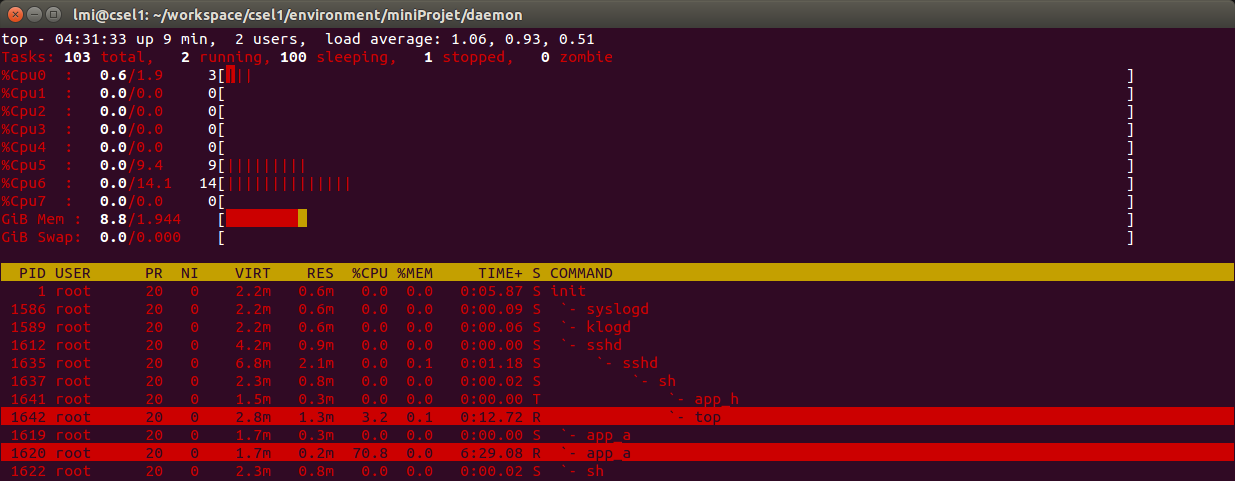
\includegraphics[width=16.5cm]{img/top3.png}
		\caption{Mesure de l'occupation du processeur}
		\label{top3}
	\end{center}
\end{figure}
On peut constater que nos différentes parties occupent peu de place au niveau du processeur.

\subsection{Points à améliorer}
Comme pour le projet sur le fan control, les boutons n'ont pas d'anti-rebond, ils restent parfois bloqués dans le mauvais état.\\
Les valeurs de duty cycle et le mode géré par la carte d'extension et par l'application utilisateur ne sont pas synchronisés. Les deux tâches sont faites dans deux processus différents. Le duty cylce incrémenté par les boutons n'est pas identique au duty entré dans l'application utilisateur. Cela ne pose pas de problème particulier au niveau de l'utilisation, mais pourrait être faire en faisant par exemple un pipe entre les deux processus pour synchroniser les données.\\